% *********************************************************************
%    2016年 学士論文
% *********************************************************************
\documentclass[12pt,a4paper,titlepage]{jreport}

% 基本的なセット
\usepackage{graphicx,moreverb,amsmath,amsthm,amssymb}

% カスタム
\usepackage{comment,url}

% ソースコード掲載用
%\usepackage{listings,jlisting,ascmac,verbatim}

%\lstset{%
%  language={HTML},
%  % basicstyle={\footnotesize}
%  basicstyle={\small},%
%  identifierstyle={\small},%
%  commentstyle={\small\itshape},%
%  keywordstyle={\small\bfseries},%
%  ndkeywordstyle={\small},%
%  stringstyle={\small\ttfamily},
%  frame={tb},
%  % frame=trBL,
%  breaklines=true,
%  columns=[l]{fullflexible},%
%  numbers=left,%
%  xrightmargin=0zw,%
%  xleftmargin=3zw,%
%  numberstyle={\scriptsize},%
%  stepnumber=1,
%  numbersep=1zw,%
%  lineskip=-0.5ex%
%}

\setlength{\topmargin}{5pt}
\setlength{\oddsidemargin}{15pt}
\setlength{\evensidemargin}{15pt}
\setlength{\marginparwidth}{10pt}
\setlength{\textwidth}{30em}
\addtolength{\textwidth}{50pt}
\addtolength{\textheight}{50pt}

%------  ヘッダの飾り ------
\makeatletter
  \def\ps@testheadings{\let\@mkboth\markboth
  \def\@oddfoot{\hfil \rm\thepage \hfil}\def\@evenfoot{}
  \def\@oddhead{
   \underline{\hbox to 140mm{\hfil\rightmark}}}%\textwidth{\hfil\rightmark}}}
  \def\chaptermark##1{\markright {\uppercase{\ifnum \c@secnumdepth
  >\m@ne
  \@chapapp \ \fi ##1}}}}
\makeatother

\pagestyle{bothstyle}
\renewcommand{\bibname}{参考文献}
%--------------------------
\begin{document}
\pagenumbering{roman}
\baselineskip 22pt
%--------- 表紙 -----------------
\title{
\flushleft{\vspace{-3cm}\small{平成28年度~~卒業研究}}\\\vspace{3.5cm}
\center{{\huge \bf 機能語に注目した\\音声合成朗読システムのための感情推定}}\vfill}
\author{
\rightline{東京理科大学~~理工学部~~経営工学科}\\
\rightline{西山研究室~~7413069~~恒川~~泰輝}\\
\rightline{}\\
\rightline{指導教員~~~西山~~裕之}}
\date{}
\maketitle

%--------------------------------------------------
%     概要
%--------------------------------------------------
\chapter*{学士論文概要}
\addcontentsline{toc}{chapter}{学士論文概要}

%社会的背景
近年,従来の書籍の他に電子書籍など様々な書籍の楽しみ方が広がっている.
朗読音声を収録したオーディオブックが近年インターネットを介して気軽にダウンロードして楽しめる環境が整ったことなどによりアメリカとカナダの市場規模が急速に拡大している.
日本においても今後さらに普及する可能性がある.
しかし,オーディオブックは書籍から音声化する際にはコストが電子書籍にくらべて10倍ほどかかっており2〜3ヶ月ほどかかると言われている.

%技術的・研究的背景・問題
そこで,電子書籍から人間の音声を人工的に作り出す音声合成技術を用いて機械で自動的に朗読するシステムの研究が行われている.
近年の音声合成技術を用いれば喜怒哀楽といった感情を指定することで感情豊かな音声を合成できる.
しかし,これらのパラメタ人手で設定する必要があり,小説といった膨大な文章に対して都度人手でパラメタ調整を行うのは手間がかかる.

%目的
そこで本研究では未知の文に対しその文を読み上げるときの感情として最適なものを推測することを目的とする.
これにより自然な朗読システムが可能が実現可能になり,オーディオブック作成時のコスト削減が期待される.

%目的を達成するための手法
本研究では,文にどの単語が含まれているかという出現情報をもとに機械学習技術を用いて感情を推定する.
名詞,動詞,形容,形容動詞は内容語とよばれるが物語に依存する可能性が高いため,内容を除いた機能語を用いることで内容に依存しない分類器を生成できる.
このため内容語を無視して機能語のみを用いて学習し感情の推定を行う.
%実験手法の正しさの確認
本研究では,4つに感情をクラス分けをする.
本手法の正しさを確認するために,まず一つの文にそれぞれ4つの感情で音声を合成し,Webアンケートシステムを用いて被験者にこれらの音声を聞いてもらい,どの感情が最も適しているか判定してもらう.
このように生成された学習データを用い交差検証を行うことで本手法の分類性能を評価する.

%-----------目次---------
\tableofcontents
\newpage
\listoffigures
\newpage
\listoftables
%\newpage
%---------------------------
\newpage

\newenvironment{indention}[1]{\par
\addtolength{\leftskip}{#1}
\begingroup}{\endgroup\par}

\pagenumbering{arabic}
%---------------------------

%--------------------------------------------------
%     第1章 序論
%--------------------------------------------------
\begin{comment}
- 主張
オーディオブックの作成にあたり
- 朗読システム
  - オーディオブック
    - 市場の拡大
  - 電子書籍
  - 課題
- 音声合成
  - 感情を込められる
  - 人手によるパラメタ調整
- 感情推定
  - EmotionML
\end{comment}

\chapter{序論}

%序論ではまず,本論文の背景としてオーディオブックと音声合成について解説する.


\section{背景}

%\subsection{音声合成}
%音声合成とは,人間の音声を人工的に作り出すことである.音声合成技術は文字を読むことが困難な障害者,外国人や幼児などに画面読み上げソフトとして長く利用されてきており,言葉を発することが困難な人が代替手段として利用することも多い.さらに,21世紀に入ってからは家電製品の音声ガイダンスや公共交通機関のアナウンス,ロボットの発話用途などとして広く使用されるようになっている.
%
%
%\subsection{オーディオブック}
%オーディオブックとは主に書籍を朗読したものを録音した音声コンテツのことである.
%アメリカを中心に市場規模が拡大している.
%もともと車社会のアメリカなどの国では早期から市場が確立していたが,近年インターネットを介して気軽にダウンロードして楽しめる環境が整ったことなどによりアメリカとカナダの市場規模が2015年には前年比21\%拡大している.
%また日本においても定額配信サービスが開始されており,今後さらに普及する可能性がある.しかしながら,このようなオーディオブックは書籍から音声化する際に手間やコストが電子書籍にくらべて10倍ほどかかっており2〜3ヶ月ほどかかると言われいる.
%
%
%\section{本論文の目的}
%音声合成技術を用いて人手で行っている朗読作業を根源的な目的である.これまでの音声合成研究の結果,単に情報を伝達する目的では十分な音質が確立されている.しかし,従来の音声合成は一文やフレーズの読み上げでは高品質な音声を実現している一方で書籍データのような長い文章では平板で淡々とした読み上げになってしまい,感情的あるいは情緒的な表現を多く含む小説などの朗読を聞くには不十分である.
%近年になって, 喜怒哀楽といった感情の種類をパラメタとして与え表現豊かな音声を合成できるソフトが販売されている.しかし,これらのパラメタは文または単語ごとに人手で設定する必要がある.短い文章など限られた場合は容易であるが, 小説といった膨大な文章に対して都度人手でパラメタ調整を行うのは大変手間がかかる.
%そこで,本研究では文章から読み上がる感情として最適なものを推測することを目的とする.


%社会的背景
近年,従来の書籍の他に電子書籍など様々な書籍の楽しみ方が広がっている.
その中で,書籍の朗読は専門のナレーターによる朗読音声を収録したオーディオブックが知られている.
オーディオブックはアメリカを中心に市場規模が拡大している.
もともと車社会のアメリカなどの国では早期から市場が確立していたが,近年インターネットを介して気軽にダウンロードして楽しめる環境が整ったことなどによりアメリカとカナダの市場規模が2015年には前年比で約21\%拡大している\cite{wsj}.
日本においても定額配信サービスが開始されており,今後さらに普及する可能性がある.


しかし,このようなオーディオブックは書籍から音声化する際には手間やコストが電子書籍にくらべて10倍ほどかかっており2〜3ヶ月ほどかかると言われている.\cite{ueda}

%技術的・研究的背景・問題
そこで,電子書籍から人間の音声を人工的に作り出す音声合成技術を用いて機械で自動的に朗読するシステムの研究が行われている.
近年の音声合成技術を用いれば喜怒哀楽といった感情を指定することで感情豊かな音声を合成できる.
しかし,これらのパラメタは文もしくは単語ごとに人手で設定する必要がある.
短い文章など限られた場合は容易であるが,小説といった膨大な文章に対して都度人手でパラメタ調整を行うのは手間がかかる.

%目的
そこで本研究では未知の文に対しその文を読み上げるときの感情として最適なものを推測することを目的とする.
これにより自然な朗読システムが可能が実現可能になり,人手での手間やコストをかけずにオーディオブックを作成できるようになることが期待される.

%目的を達成するための手法
本研究では,文にどのような単語が含まれているかという出現情報をもとに機械学習技術を用いて感情を推定する.
名詞,動詞,形容,形容動詞は内容語とよばれるが物語に依存する可能性が高いため,内容を除いた機能語を用いることで内容に依存しない分類器を生成できる.
このため内容語を無視して機能語のみを用いて学習し感情の推定を行う.
セリフのみに限らずすべての文を対象に,出現情報から機能語に絞った感情推定を行っている研究は筆者の知る限り存在しない.

%実験手法の正しさの確認
本研究では,先行研究と同様にNormal,Happy,Sad,Angryの4つに感情をクラス分けする.
本手法の正しさを確認するための実験として,まず一つの文にそれぞれ4つの感情で音声を合成する.
そしてWebのアンケートシステムを用いて,被験者にこれらの音声を実際に聞いてもらい,その文を読み上げる際にどの感情が最も適しているか判定してもらう.
このように生成された学習データを用い交差検証を行うことで本手法の分類性能を評価する.

%\section{本論文の構成}
%本章では,本論文の背景となる。。。について説明した.そのうえで,。。。のニーズと課題につ いて説明し,それを踏まえ。。。。概要に触れた後,本論 文の目的を述べた.第二章では既存の関連する研究について述べる.また第三章では本論文が提案する手法の詳細を述べ,第四章でその具体的な実装につい て説明する.そのうえで第五章で提案手法の効果を測定するために行なった実験の結果と考察を述べ,六章でその結論と今後の展望について述べる.


%--------------------------------------------------
%     第2章 関連研究
%--------------------------------------------------
\chapter{関連研究}
本研究に関連する過去の研究について述べる.

感情を考慮した音声合成の研究として大谷\cite{otani}らは共有感情モデルを構築してる.
このモデルを用いることで音声を合成する際に感情を表出させることが可能である.
しかし,感情パラメタ自体は人手で与える必要がある.
本研究と組み合わせることで自動的に感情を推定しパラメタを与えることで,文そのもののみで感情豊かな音声合成が可能となる.

吉田ら\cite{yoshida}は自然な朗読システムのために文内・文末表層情報に着目している.
文内情報(命令,否定,意志等)と文末情報(「〜ある」,「〜いる」,「〜んだ」等)をカテゴリー分けし,実際の朗読音声を元に文間ポーズと基本周波数,話速のモデル化を行うことで推定を実現している.
しかし,この研究はあくまで自然な朗読システムの構築を目的としてるため,感情が考慮されてるとは言えない.
本研究では物語から喜怒哀楽といった感情を推定することで,感情豊かな朗読システムの実現を目指している.

布目ら\cite{fume}はポーズ情報の推定と感情表現の推定を行っている.
ポーズ推定では,タイトルや章立て構造といった文章の論理要素に応じてポーズ長を推定し,ポーズを挿入する.
感情推定では「喜び」「怒り」「悲しみ」及び「平静」の各感情を付与した学習データを作成する.
ナイーブベイズを用いて学習を行い,推定ではスコアを算出し最もスコアの高い感情を文に付与する.
その推定をもとに,文ごとに韻律辞書や音声制御用パラメタを切り替えて読み上げる.
しかしながら,感情を付与する対象はセリフのみであり,本研究ではセリフ以外の文についても感情を付与する.


%--------------------------------------------------
%     第3章 提案手法
%--------------------------------------------------
\chapter{提案手法}

本章では提案する手法の詳細について説明する.

\section{提案手法の概要}
\begin{figure}[ht]
  \begin{center}
    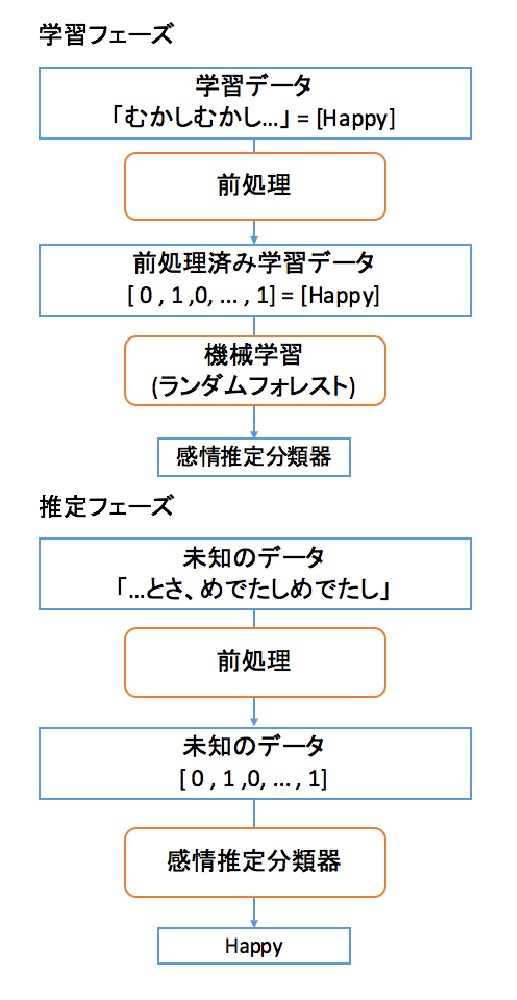
\includegraphics[clip,width=7.0cm]{fig/method-2.eps}
    \caption{提案手法の概要}
    \label{fig:method}
  \end{center}
\end{figure}

提案手法の概要を図\ref{fig:method}に示す.
本手法では,物語中のすべての文に対し文中に含まれる単語の出現を手がかりに朗読に最も適切もしくは自然と感じる感情を推定する.
感情のクラスはNormal,Happy,Sad,Angryの4種類とした.
まず,学習データとして各文に,それぞれ適切と思われる感情を人手で割り当てたものを用意する.
これに対し前処理を行いランダムフォレストを用いて学習を行う.
そして未知の入力文が与えられた場合に,感情クラスの1つを自動的に推定する他クラス分類を行うのが本手法である.

\subsection{機能語のみによる推定}
本手法は,学習と推定の際に文から内容語(名詞,動詞,形容詞,形容動詞)を取り除き,機能語のみで推定を行う.
なぜならば,未知の物語の感情を推定を目的としているため,学習データが特定の物語に依存していては推定精度が低くとなると考えられるからである.
例えば「鬼」がネガティブに描かれている物語を学習データとして,別の「鬼」がポジティブに描かている物語を推定した場合にネガティブな感情に推定されてしまう恐れがある.
一方,機能後は「しまう」や「ところが」など,朗読時の抑揚などに関係すると考えられる重要な助詞やや接続詞を含む.
したがって,内容語を排除し排除し,機能語のみで推定を行う.

\subsection{前処理}
\begin{figure}[ht]
  \begin{center}
    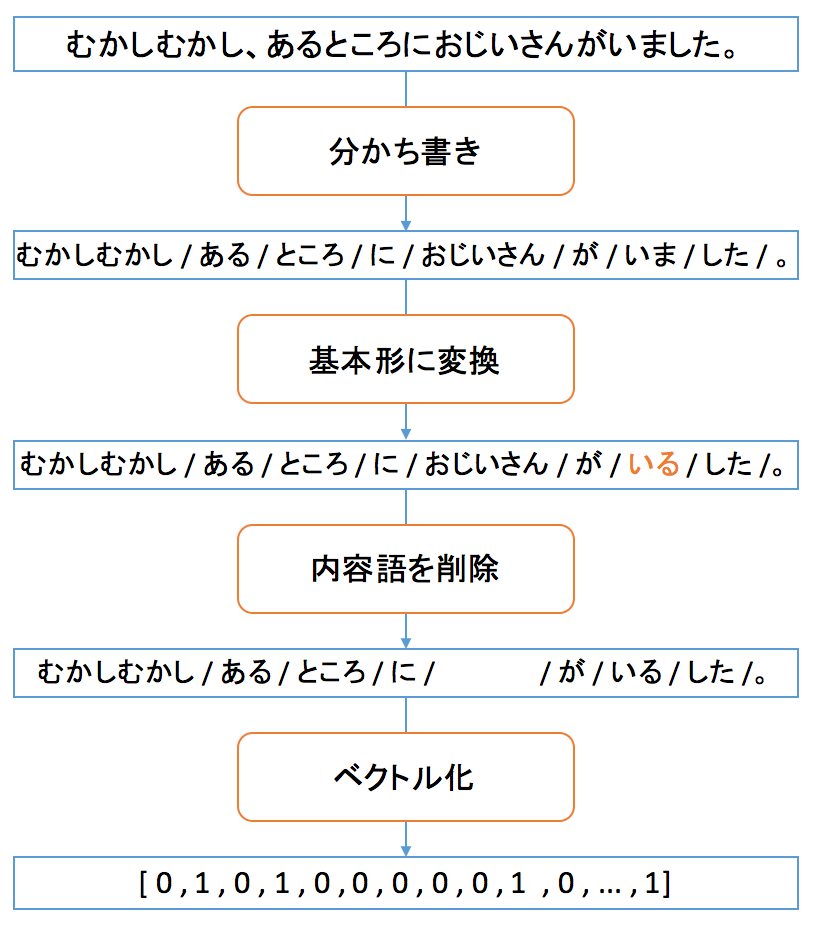
\includegraphics[clip,width=7.0cm]{fig/method.eps}
    \caption{前処理の手順}
    \label{fig:pre}
  \end{center}
\end{figure}

前処理の概要を図\ref{fig:pre}に示す.
まず,物語の文章を文に分ける際は,基本的に句点で区切る.
カギ括弧で囲まれているセリフ部分はカギ括弧で区切り,カギ括弧内のセリフについても句点で区切る.
次に,形態素解析を行い単語ごとに分割しそれぞれの単語を基本形に変換する.
そして,形態素解析の結果から内容語を削除し機能語のみにする.
最後に,文中に単語が含まれるか否かを示すベクトル(Bag-of-words)に変換する.

\subsection{分類器の生成}
一般に,入力データに対して,予め定義された複数のクラスから一つを推定する手法としては機械学習の教師あり学習が適応できる.
本研究では,その1つであるランダムフォレストを用いて推定を行う.
ランダムフォレストは複数の決定木を用いて識別などを行うアンサンブル学習アルゴリズムである.
また,精度を向上させるために,正確度を指標としてグリットサーチを用いて最適なパラメタを探索する.
%TODO-me
%本研究で調整したパラメタはの\ref{parameter}通りである.


%--------------------------------------------------
%     第4章 実装
%--------------------------------------------------
\chapter{データセット}
本章では実験に用いる教師データを収集するためのシステムや集計手法について説明する.
教師データの作成手順を図\ref{fig:enquete}に示す.
本研究では,まず物語文を元に各感情を指定した音声データを生成し,Webのアンケートシステムを用いて複数の被験者に評価してもらい,学習データを作成する.

\begin{figure}[hb]
  \begin{center}
    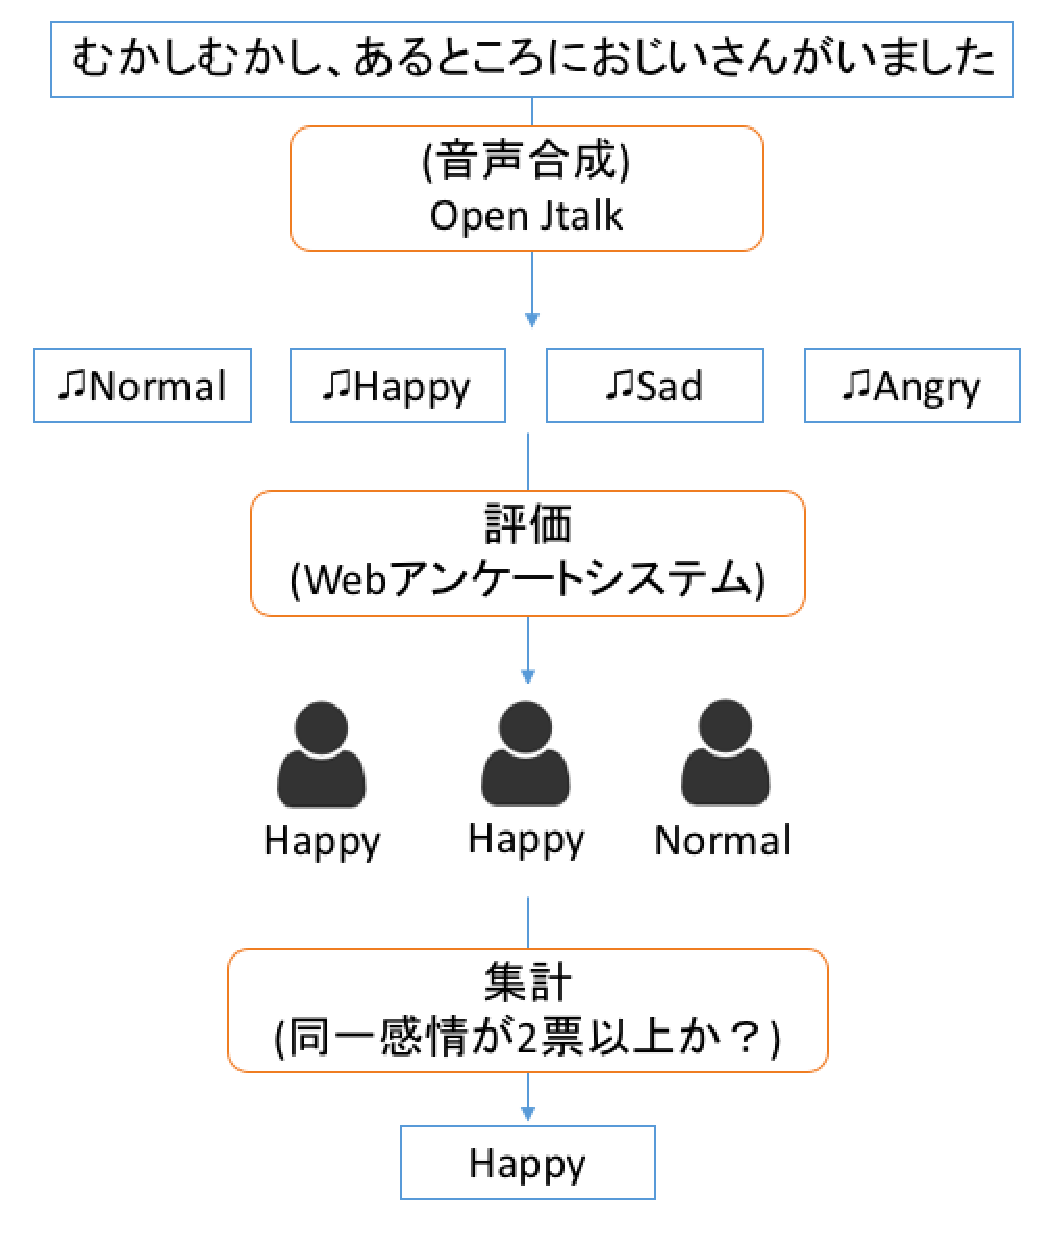
\includegraphics[clip,width=10.0cm]{fig/enquete.eps}
    \caption{学習データの作成手順}
    \label{fig:enquete}
  \end{center}
\end{figure}

\section{物語文章}
本実験では物語データとして,青空文庫\cite{aozora}にある5つの物語を用いる.
青空文庫とは,著作権が消滅した作品や著者が許諾した作品のテキストを公開しているインターネット上の電子図書館である
今回は文体を近づけるために同じ訳者の童話を中心に「白雪姫」,「赤ずきんちゃん」,「浦島太郎」,「ジャックと豆の木」,「ヘンゼルとグレーテル」を用いた.
%TODO 著者などを添えた表

\section{音声データの作成}
\subsection{前処理}
\ref{subsec:divide}で述べたように物語の文章を文に分ける.
朗読システム実現するためにはこの処理も自動化する必要がある.
また,青空文庫の書籍データにはルビや改行といったHTMLタグが挿入されているためこれを除く必要がある.
プログラミング言語Rubyを用いて,これらの処理を実装した.
これらの処理の例を\ref{fig:aozora-convert}に示す.

\begin{figure}[hb]
  \begin{center}
    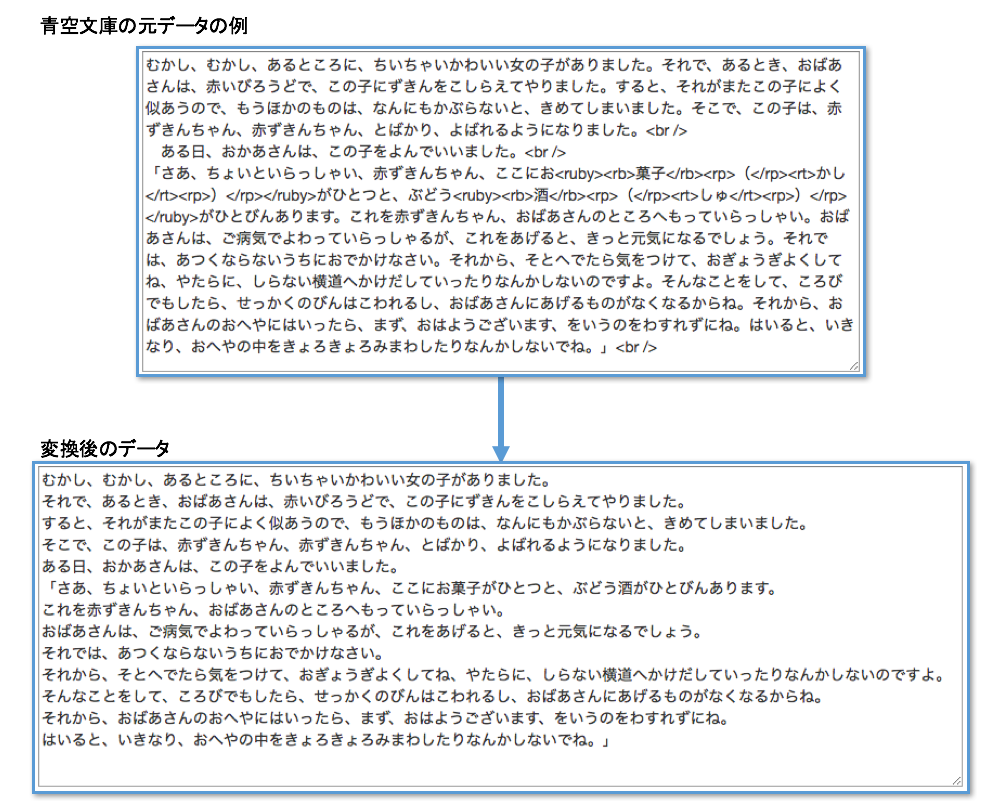
\includegraphics[clip,width=16.0cm]{fig/aozora-convert.eps}
    \caption{青空文庫データの文分割とタグ削除処理}
    \label{fig:aozora-convert}
  \end{center}
\end{figure}

\subsection{音声合成ソフト}
本研究では音声合成にオープンソフトのOpen JTalk\cite{jtalk}を用いる.
Open Jtalkは日本語テキスト向けのHMM型の音声合成のオープンソースのソフトウェアである.
\ref{hmm-emotion}で述べた通りHMM型音声合成手法は少ない学習データで感情表現が可能になっている.
また,再現実験を考慮し広く利用が可能なオープンソースソフトウェアであるOpen Jtalkを用いた.


音声波形データにはMMDAgent\cite{mei}にあるMeiのサンプルを用いた.
この音声波形データは1人の女性の848文の音声サンプルをもとに作成されている.
そのうち,503文は音声波形作成に広く用いられている用いられるATR音素バランス503文\cite{atr}であり,残りのうち215文は普通の発話スタイルで,残る75文は4つの感情(Angry, Bashful, Happy, Sad)の発話スタイルで収録されている.
それゆえ,MMDAgentにはNormal, Angry, Bashful, Happy, Sadの5つの音声波形データが用意されている.
本研究では布目ら\cite{fume}などの研究に従い,このうちのNormal, Angry, Happy, Sadの4つを利用した.


発音辞書にはNAIST Japanese Dictionary\cite{naist}を用いる.

\subsection{音声データファイル}
本研究では,前章のOpen JTalkとMeiの音声波形データ等を用いて,一つの文に対して4つの異なる感情表現の音声ファイルを生成する.
この音声ファイルはWAVフォーマット形式で出力される.
WAVフォーマット形式は,非圧縮形式でありリニアPCMのサンプリングデータ用のフォーマットとして扱われる.
Open JTalkの出力ではサンプルレートが48,000Hz,16bps,モノラルのWAVファイルが得られる.
%TODO ↑表にする??

\section{アンケートシステム}

\subsection{学習データの収集}
\begin{figure}[h]
  \begin{center}
    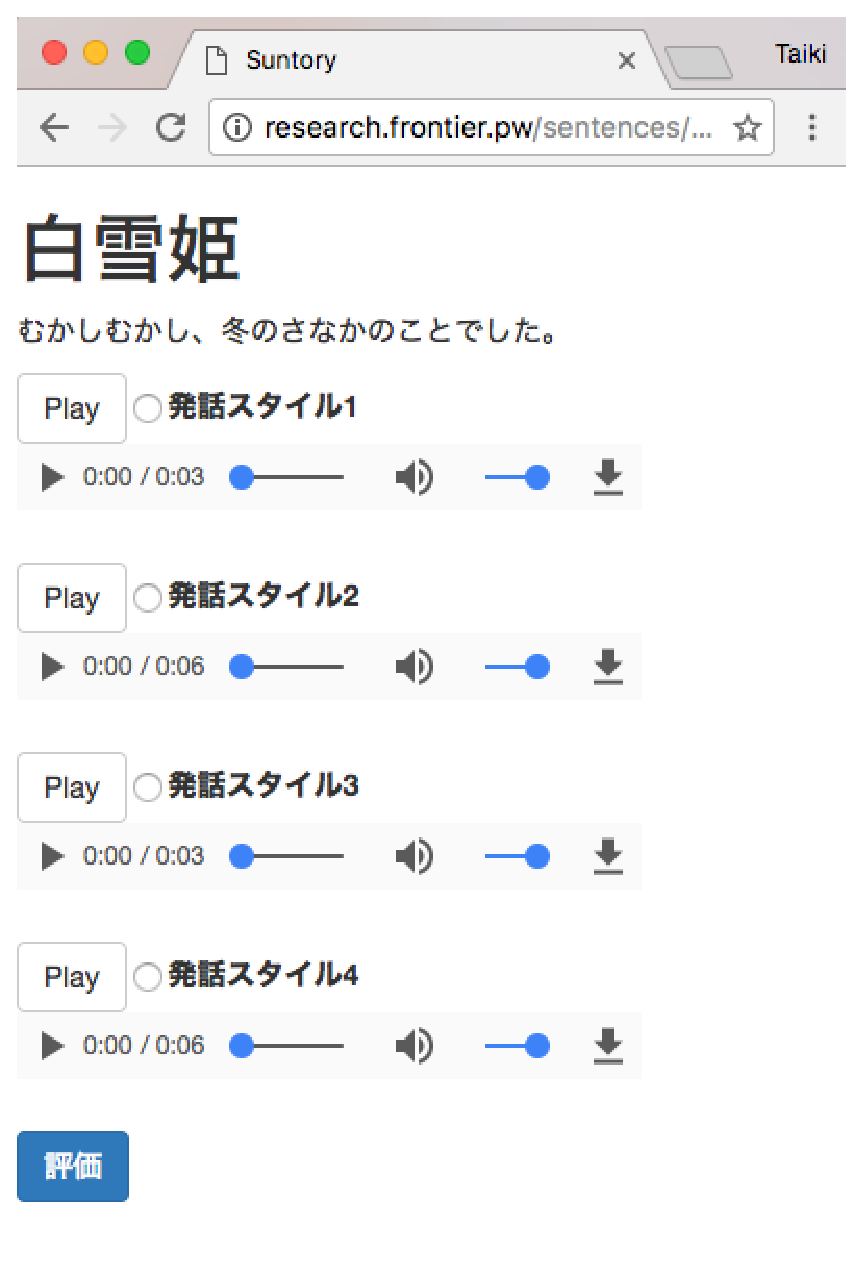
\includegraphics[clip,width=10.0cm]{fig/web.eps}
    \caption{WEBアンケートシステム画面}
    \label{fig:web}
  \end{center}
\end{figure}

本研究ではWeb上で学習データを収集するためのシステムを構築した.
そのシステム画面を図\ref{fig:web}に示す.

\subsection{}
\subsection{評価}
被験者には文ごとに各感情のパラメタで合成した音声をそれぞれ聞いてもらい内容にもっとも適切(自然)であると思われる感情を1つだけ選択してもらう.
しかし,感情は主観的な尺度であるため一人だけの評価では信頼性が低い.
そこで,一文に対して同じ感情の評価が二票集まった時点で,その文の感情を決定することとした.
したがって,同じ感情の評価が二票あるまで他の被験者に評価し続けてもらう.
被験者等に関する詳細を表\ref{enviroment}に示す.
本システム用いたサーバー機とソフトウェアの仕様は\ref{server}に示す

\begin{table}[ht]
  \begin{center}
  \caption{学習データの収集}
  \label{enviroment}
  \begin{tabular}{|c|l|}
    \hline
    被験者 & 東京理科大学の学部生及び大学院生 \\ \hline
    人数 & 学部生15名,大学院生2名 \\ \hline
    取得期間 & 2017年1月9日〜25日 \\ \hline
    評価取得数 & 2641 \\ \hline
  \end{tabular}
  \end{center}
\end{table}


\begin{table}[ht]
  \begin{center}
  \caption{アンケートシステムの仕様}
  \label{server}
  \begin{tabular}{|c|l|}
    \hline
    被験者 & 東京理科大学の学部生及び大学院生 \\ \hline
    人数 & 学部生15名,大学院生2名 \\ \hline
    取得期間 & 2017年1月9日〜25日 \\ \hline
    評価取得数 & 2641 \\ \hline
  \end{tabular}
  \end{center}
\end{table}

\section{集計方法}

\section{得られた学習データ}
\begin{table}[ht]
 \centering
  \caption{学習データ(物語別)}
  \vspace{0.3\baselineskip}
  \scalebox{0.8}{
  \begin{tabular}{|c|c|c|} \hline
    タイトル & 文数(セリフ) & 評価確定数(セリフ) \\ \hline \hline
    白雪姫 & 287 (90) & 258 (86)   \\ \hline
    赤ずきんちゃん & 109 (54) & 108 (54)   \\ \hline
    浦島太郎 & 206 (48) & 78 (26)   \\ \hline
    ジャックと豆の木 & 206 (49) & 78 (26)   \\ \hline
    ヘンゼルとグレーテル & 319 (114) & 260 (90)   \\ \hline\hline
    合計 & 1096 (364) & 765 (283) \\ \hline
  \end{tabular}
  }
  \label{sentence-count}
\end{table}

\begin{table}[ht]
 \centering
  \caption{学習データ(感情別)}
  \vspace{0.3\baselineskip}
  \scalebox{0.90}{
  \begin{tabular}{|c|c|c|} \hline
    感情 & 全文 & セリフのみ  \\ \hline \hline
    Normal & 459  & 63  \\ \hline
    Happy & 134 & 110 \\ \hline
    Sad & 99  & 60  \\ \hline
    Angry & 73  & 50  \\ \hline \hline
    合計 & 765 &  283 \\ \hline
  \end{tabular}
  }
  \label{emotion-count}
\end{table}

学習データの概要を表\ref{sentence-count}と表\ref{emotion-count}に示す.
全体で評価が確定したものは全体で69.8\%であった.
全文とセリフのみに絞った場合の比較を行う.
得られた学習データは表\ref{emotion-count}の通り,Normal以外の感情はセリフに多く含まれることがわかる.
したがってセリフの感情推定の精度を上げることで全体の精度をあげることができることがわかる.
全文にくらべセリフのみを対象とした場合はより均等に感情が別れているため分類がより難しい.




%--------------------------------------------------
%     第5章 評価と考察
%--------------------------------------------------
\chapter{評価}

本章では提案手法を具体的に実装したシステムを用いて,主要コンテンツの抽出性能を評価するために行なった実験の概要と結果について述べる.

\section{評価目的}


%--------------------------------------------------
%     第6章 結論
--------------------------------------------------
\chapter{結果}

%TODO F値最適の結果
%TODO 説明も増やす


\subsection{グリッドサーチ}
\begin{table}[ht]
 \centering
  \caption{ランダムフォレストのグリットサーチの結果}
  \vspace{0.3\baselineskip}
     \scalebox{0.75}{
  \begin{tabular}{|c|c|c|c|c|} \hline
  パラメタ名 & 全文 & \shortstack{全文\\(機能語のみ)} & セリフ & \shortstack{セリフ\\(機能語のみ)}\\ \hline \hline
  ceriterion & entropy & entropy & entropy & entropy\\ \hline
  min\_samples\_leaf & 12 & 8 & 3 & 8\\ \hline
  n\_estimators & 80 & 250 & 30 & 30\\ \hline
  max\_features & None & None & None & None\\ \hline
  min\_samples\_split & 12 & 10 & 3 & 10\\ \hline
 max\_depth & 17 & 20 & 20 & 15\\ \hline
  \end{tabular}}
  \label{gs-rf}
\end{table}

\begin{table}[ht]
 \centering
  \caption{SVMのグリットサーチの結果}
  \vspace{0.3\baselineskip}
     \scalebox{0.8}{
  \begin{tabular}{|c|c|c|c|c|} \hline
  パラメタ名 & 全文 & \shortstack{全文\\(機能語のみ)} & セリフ & \shortstack{セリフ\\(機能語のみ)}\\ \hline \hline
  kernel & sigmoid & sigmoid & poly & rbf\\ \hline
  gamma & 0.001 & 0.001 & 3 & 0.001\\ \hline
  C & 100 & 100 & 1000 & 1\\ \hline
  \end{tabular}}
  \label{gs-svm}
\end{table}

グリッドサーチの結果を表\ref{gs-rf}表と表\ref{gs-svm}に示す.
それぞれの場合で値が大きく異なるパラーメタが得られる場合があった.

\subsection{評価結果}
\begin{table}[ht]
 \centering
  \caption{ランダムフォレストでの結果}
  \vspace{0.3\baselineskip}
  \scalebox{0.9}{
  \begin{tabular}{|l|c|c|c|c|} \hline
    対象 & 正確度 & 適合率 & 再現率 & F値  \\ \hline \hline
    全文 & 0.82 & 0.57 & 0.64 & 0.57  \\ \hline
    全文(機能語) & 0.82 & 0.54 & 0.64 & 0.57   \\ \hline
    セリフのみ & 0.70 & 0.37 & 0.40 & 0.37   \\ \hline
    セリフのみ(機能語) & 0.70 & 0.35 & 0.40 & 0.34  \\ \hline
  \end{tabular}
  }
  \label{res-rf}
\end{table}

\begin{table}[ht]
 \centering
  \caption{SVMでの結果}
  \vspace{0.3\baselineskip}
  \scalebox{0.9}{
  \begin{tabular}{|l|c|c|c|c|} \hline
    対象 & 正確度 & 適合率 & 再現率 & F値  \\ \hline \hline
    全文 & 0.82 & 0.57 & 064 & 0.59   \\ \hline
    全文(機能語) & 0.80 & 0.36 & 0.60 &  0.45 \\ \hline
    セリフ & 0.70 & 0.38 & 0.22 & 0.22   \\ \hline
    セリフ(機能語) & 0.70 & 0.15 & 0.39 & 0.22   \\ \hline
  \end{tabular}
  }
  \label{res-svm}
\end{table}

ランダムフォレストとSVMの結果を表\ref{res-rf}と表\ref{res-svm}に示す.
なお(機能語)とは学習,推定時に機能語のみを用いた場合を示す.
全体としてF値は高くない結果となった.
特にSVMの場合はSVMでは,全文に機能語を絞らずに分類を行った場合を除く他のすべての場合で,推定が一つの感情に偏ってしまった.

\subsection{考察}
全体としてのF値は高くない結果となった.
原因として学習データが少ないことや出現を示すベクトルの形式に問題がある可能性がある.
また,グリットサーチを正確度を基準に行ってしまったためF値を基準にやり直す必要がある.

ランダムフォレストとSVMを比較する.
SVMでは,全文に機能語を絞らずに分類を行った場合を除く他のすべての場合で,推定が一つの感情に偏ってしまった.
したがって,本研究の目的のためにはSVMよりランダムフォレストの方が有用であると言える.

機能語に絞った場合ととそうでない場合を比較する.
ランダムフォレストの値ではほぼ同じもしくは機能語に絞らない方がわずかに良い結果が得られている.
これは,学習データに用いた物語が5つと少ないことやleave-one-outを用いたことで推定する文と同じ物語の文を用いて学習を行っているからであると考えられる.
したがって,機能語だけでも感情の推定を行える可能性はまだある.
実際の運用では未知の物語の文に対して推定を行うので,機能語だけの学習・推定の方が精度が高い推定が行えるかもしれない.
この検証を行うためには物語数を増やし学習データを増やした上で,leave-one-outではなく一つの物語をテストデータして他の物語を学習データとして検証を行う必要がある.
また,決定木を用いて各単語の重要度を算出することで,機能語が感情推定にどれほど寄与するのか確認することができる.


全体で評価が確定したものは全体で69.8\%であった.
全文とセリフのみに絞った場合の比較を行う.
得られた学習データは表\ref{emotion-count}の通り,Normal以外の感情はセリフに多く含まれることがわかる.
したがってセリフの感情推定の精度を上げることで全体の精度をあげることができることがわかる.
全文にくらべセリフのみを対象とした場合はより均等に感情が別れているため分類がより難しい.



%--------------------------------
%     参考文献
%--------------------------------
\markright{参考文献}
\begin{thebibliography}{99}

%TODO 順番確認
% http://ci.nii.ac.jp/naid/110009971766
\bibitem{wsj} Jennifer Maloney,"The Fastest-Growing Format in Publishing: Audiobooks",http://www.wsj.com/articles/the-fastest-growing-format-in-publishing-audiobooks-1469139910,Wall Steet Journal
\bibitem{cnet} 佐藤和也,"高い継続率は「耳がさみしくなるから」--オトバンクに聞くオーディオブック市場と利用動向",https://japan.cnet.com/article/35076656/
\bibitem{ueda} 上田渉,"「耳で聴く読書文化」を築く",http://www.ajec.or.jp/interview\_width\_ueda1/,一般社団法人日本編集制作協会
\bibitem{sugifuji} 杉藤美代子; 大山玄. 朗読におけるポーズと呼吸―息継ぎのあるポーズと息継ぎのないポーズ―. 音声言語. 1990.
\bibitem{yoshimura} YOSHIMURA, Takayoshi. Simultaneous modeling of phonetic and prosodic parameters, and characteristic conversion for HMM-based text-to-speech systems. 2002. PhD Thesis. Nagoya Institute of Technology.
\bibitem{iida} 飯田朱美, and 安村通晃. "感情表現が可能な合成音声の作成と評価." 情報処理学会論文誌 40.2 (1999): 479-486.
\bibitem{tsuduki} 都築亮介, et al. HMM 音声合成における感情表現のモデル化 (合成, 韻律, 生成, 一般). 電子情報通信学会技術研究報告. SP, 音声, 2003, 103.264: 25-30.
\bibitem{habe} 波部斉,”ランダムフォレスト”,情報処理学会研究報告 2012

\bibitem{yoshida} 吉田有里,奥平康弘,田村直良,”音声合成による朗読システムに関する研究”,情報科学技術フォーラム講演論文集,2009:p337-380
\bibitem{otani} 大谷大和, et al. "HMM に基づく感情音声合成のための共有感情付与モデル (オーガナイズドセッション 「文脈や状況に合った発声を実現する音声合成技術及び周辺技術」, 合成, 韻律, 生成, 音声一般)." 電子情報通信学会技術研究報告. SP, 音声 114.303 (2014): 13-18.
\bibitem{fume} 布目光生,鈴木優,森田眞弘,”自然で聞きやすい電子書籍読上げのための文書構造解析技術,東芝レビュー,2011:p32-35
\bibitem{aozora} 青空文庫,http://www.aozora.gr.jp/
%TODO 他の文も
%\bibitem{shirayuki} グリム,菊池寛訳,”白雪姫”,http://www.aozora.gr.jp/cards/001091/files/42308\_17916.html

%ちゃんとした形式に直す
\bibitem{jtalk} 大浦 圭一郎,酒向 慎司, 徳田 恵一,”日本語テキスト音声合成システム Open JTalk”,日本音響学会春季講論集,2010:p343-344
\bibitem{mecab} "MeCab: Yet Another Part-of-Speech and Morphological Analyze",http://taku910.github.io/mecab/
\bibitem{naist} "NAIST Japanese Dictionary",http://naist-jdic.osdn.jp/
\bibitem{mei} LEE, Akinobu; OURA, Keiichiro; TOKUDA, Keiichi. MMDAgent—A fully open-source toolkit for voice interaction systems. In: Acoustics, Speech and Signal Processing (ICASSP), 2013 IEEE International Conference on. IEEE, 2013. p. 8382-8385.
\bibitem{atr} 磯健一; 渡辺隆夫; 桑原尚夫. 音声データベース用文セットの設計. 昭 63 年春音講論, 1988, 2-2.
\bibitem{ruby} "オブジェクト指向スクリプト言語 Ruby",https://www.ruby-lang.org/ja/
\bibitem{rails} "Ruby on Rails",http://rubyonrails.org/
\bibitem{sqlite} "SQLite",https://www.sqlite.org/
\bibitem{python} "プログラミング言語Python",https://www.python.jp/
\bibitem{sklearn} "scikit-learn: machine learning in Python"、http://scikit-learn.org/stable/

\end{thebibliography}


%--------------------------------
%     アペンディクス
%--------------------------------
\appendix
\chapter{WebページのURLリスト}
\vspace{-15mm}


\end{document}
